\section{Basic Tools}

The basic tool provides PIPS analysis or transformation passes. They
are available in at most two levels: basic and advanced (see
Section~\ref{paws_project}).

\subsection{Basic Level}

The basic level allows the user to try PIPS analysis or transformation
with a default setting. An example page is shown in
Figure~\ref{fig:basic_mode_screen}.

\begin{figure}[h!]
  \centering
  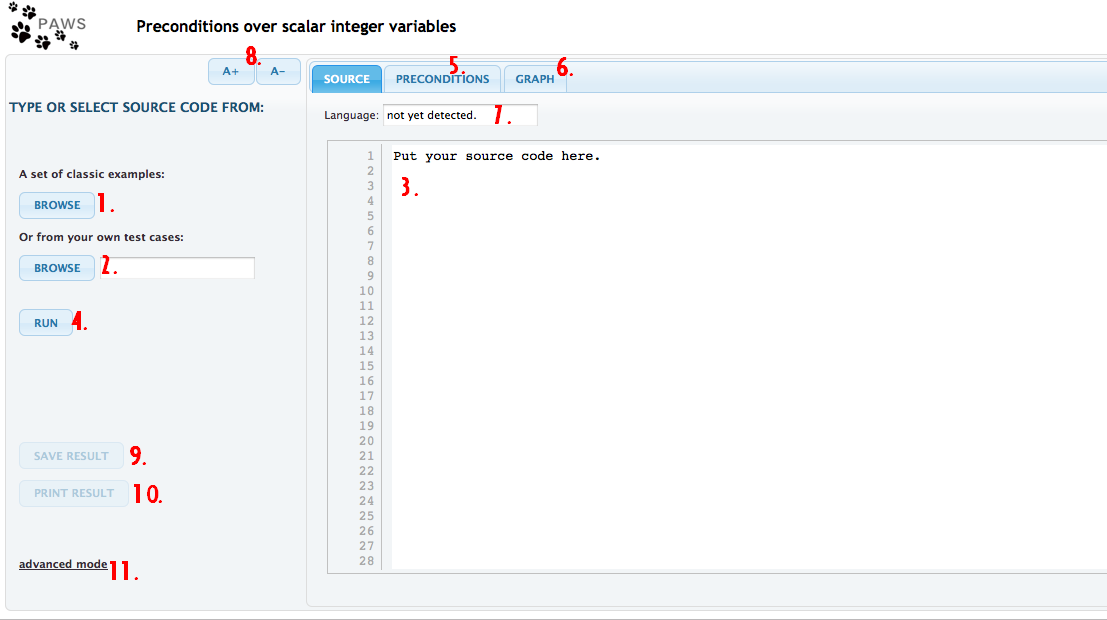
\includegraphics[width=0.8\textwidth]{reportCh4/basic_mode_screen}
  \caption{Preconditions basic level screen.}
  \label{fig:basic_mode_screen}
\end{figure}

The user can provide the source code either by loading one of supplied
examples ({\bf 1.}) or by picking it locally from his/her machine
({\bf 2.})  or by typing it in the source code window ({\bf 3.}). The
pass is launched by clicking either the button ``RUN'' ({\bf 4.}) or the
tab ``PRECONDITIONS'' ({\bf 5.}). Selecting the tab ``GRAPH'' ({\bf
  6.}) invokes the dependence graph computation and display.

After loading the source code, the language of the code is detected and
displayed in the programming language label ({\bf 7.}). In case of
inconvenience, the user can change font size used on the side by the
``A+'' and ``A-'' buttons ({\bf 8.}).

The user can save or print the results of the performed
pass. Buttons, which enable that ({\bf 9.} and {\bf 10.}),
disactivated at the beginning, are activated when the result is ready.

The link at the bottom of the page ({\bf 11.}) leads to the advanced
level mode of the same tool.

\subsection{Advanced Level}

The layout and usage of the advanced level page is very similar to the
basic one. The only difference is the possibility of setting
properties, analyses and phases (see
Figure~\ref{fig:advanced_properties}). Each setting has its
description, which is made visible when hovering the mouse over its
check button.

Boolean properties ({\bf 1.}) are set to {\bf True} or {\bf False} by
simple being checked. Integer properties ({\bf 2.}) are checked by a
default and their values can be changed by the user. After invocation
of the operation they are validated. String properties ({\bf 3.}),
analyses ({\bf 4.}) and phases ({\bf 5.}) have predefined lists of
possible values. The default one is already selected.

\begin{figure}[h!]
  \centering
  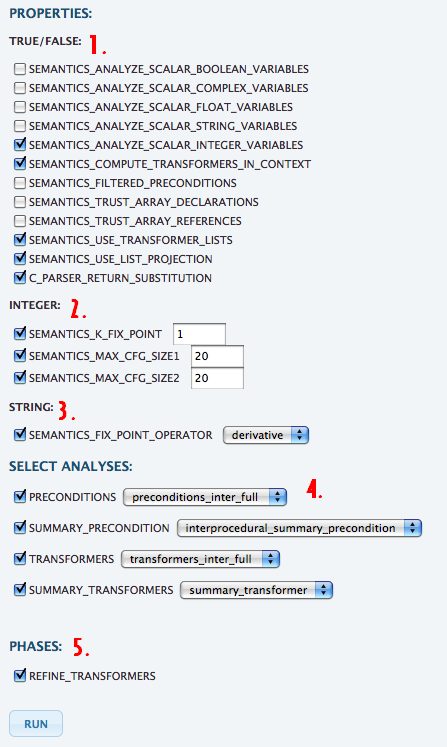
\includegraphics[width=0.5\textwidth]{reportCh4/advanced_properties}
  \caption{Forms for setting properties, analyses and phases.}
  \label{fig:advanced_properties}
\end{figure}
